\section{Примеры} 
\subsection{Ссылки на статьи}

Можно ссылаться на статью вот так:  \bibref{chirkova18}{Chirkova et al.}{2017}.

\subsection{График}

График \ref{fig:by_epochs} достаточно бессмысленный без контекста.

\begin{figure}[h!]
	\centering
	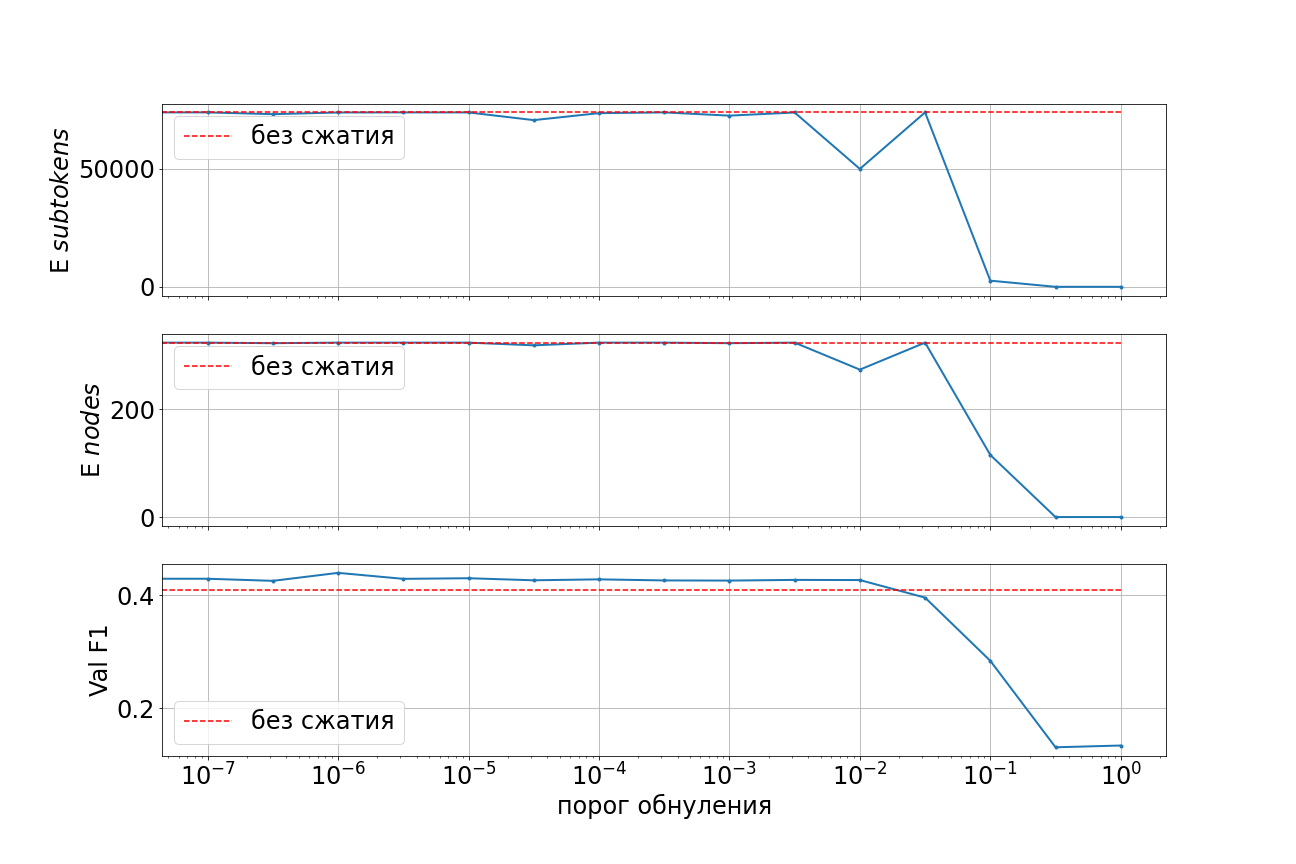
\includegraphics[width=1\textwidth]{example.png}
	\caption{Пример графика}
	\label{fig:by_epochs}
\end{figure}


\subsection{Таблица}

\begin{table}[htbp]
	\caption{Пример таблички}
	\label{table:long_epochs}
	\footnotesize
	\centering
	\begin{tabular}{lrrrrrrrr}
		\toprule
		& \multicolumn{3}{c}{$\mathsf{Val}$} &
		\multicolumn{3}{c}{$\mathsf{Test}$} \\
		\cmidrule(lr){2-4} \cmidrule(l){5-7} 
		{} &  $\mathsf{Prec}$ &  $\mathsf{Rec}$ &  $\mathsf{F1}$ &  $\mathsf{Prec}$ &  $\mathsf{Rec}$ &  $\mathsf{F1}$  &  $\mathsf{nodes}$ & $\mathsf{subtokens}$\\
		\midrule
		запуск 1    &    0.4894 &   0.3775 &  0.4263 &     0.4824 &    0.3683 &   0.4177 & 10029 & 179\\
		запуск 2    &    0.4887 &   0.3739 &  0.4237 &     0.4891 &    0.3724 &   0.4228 & 10039 & 177\\
		запуск 3    &    0.4820 &   0.3751 &  0.4219 &     0.4838 &    0.3677 &   0.4178 & 10037&	180\\
		\midrule
		\bf{среднее} &    \bf{0.4867} &   \bf{0.3755} &  \bf{0.4239} &    \bf{ 0.4851} &    \bf{0.3695} &   \bf{0.4195} \\
		\bf{дисперсия}  &    0.0041 &   0.0019 &  0.0022 &     0.0036 &    0.0025 &   0.0029 \\
		\bottomrule
	\end{tabular}
\end{table}